\documentclass{AeroStructure-ERJohnson}
\input crosslink.tex

%\usepackage{showframe}
\def\ShowFrameLinethickness{0.125pt}

%\def\harp#1{\smash{\mathord{\buildrel{\lower3pt\hbox{$\scriptscriptstyle\rightharpoonup$}}\over{#1}}}}

\makeatletter
\newenvironment{splquote}%
               {\list{}{\leftmargin18pt\listparindent\parindent\topsep-3\p@}%
                \normalsize\itemindent-5\p@\listparindent\parindent%
                \item\relax}%
               {\endlist}%
\makeatother

\myexternaldocument{App_4P}
\myexternaldocument{Ch01_4P}
\myexternaldocument{Ch02_4P}
\myexternaldocument{Ch03_4P}
\myexternaldocument{Ch04_4P}
\myexternaldocument{Ch05_4P}
\myexternaldocument{Ch06_4P}
\myexternaldocument{Ch07_4P}
\myexternaldocument{Ch08_4P}
\myexternaldocument{Ch09_4P}
\myexternaldocument{Ch10_4P}
\myexternaldocument{Ch11_4P}
%\myexternaldocument{Ch12_4P}
\myexternaldocument{Ch13_4P}
\myexternaldocument{Ch14_4P}
\myexternaldocument{Ch15_4P}
\myexternaldocument{Ch16_4P}
\myexternaldocument{Ch17_4P}
\myexternaldocument{Ch18_4P}

\begin{document}

\mainmatter

%\hbox{~}\clearpage
\setcounter{page}{331}

\setcounter{chapter}{11}

\chapter{Introduction to aeroelasticity}\label{ch12}

\section{The Collar diagram of aeroelastic forces}\label{sec12.1}

The following paragraphs are excerpted from \textit{Aeroelasticity} by R. L. Bisplinghoff, H. Ashley, and R. L. Halfman (1996).

\begin{quote}
Aeroelasticity is defined as a science which studies the mutual interaction between aerodynamic forces and elastic forces, and the influence of this interaction on airplane design. Aeroelastic problems would not exist if the airplane structure were perfectly rigid. Modern airplane structures are very flexible, and this flexibility is fundamentally responsible for the various types of aeroelastic phenomena. Structural flexibility itself may not be objectionable; however, aeroelastic phenomena arise when structural deformations induce additional aerodynamic forces. Such interactions may become smaller and smaller until a condition of stable equilibrium is reached, or they may tend to diverge and destroy the structure.

The term aeroelasticity, however, is not completely descriptive, since many important aeroelastic phenomena involve inertial forces as well as aerodynamic and elastic forces. We shall apply a definition in which the term aeroelasticity includes phenomena involving interactions among inertial, aerodynamic, and elastic forces, and other phenomena involving interactions between aerodynamic and elastic forces. The former will be referred to as \textit{dynamic} and the latter as \textit{static} aeroelastic phenomena.

Collar has ingeniously classified problems in aeroelasticity by means of a triangle of forces. Referring to Fig.~1-1
[figure~\ref{fig12.1} below], the three types of forces, aerodynamic elastic, and inertial are represented by the symbols \textit{A}, \textit{E}, and \textit{I}, respectively, are placed at the vertices of a triangle. Each aeroelastic phenomenon can be located on the diagram according to its relation to the three vertices. For example, dynamic aeroelastic phenomena such as flutter \textit{F}, lie within the triangle, since they involve all three types of forces and must be bonded to all three vertices. Static aeroelastic phenomena such as wing divergence, \textit{D}, lie outside the triangle on the upper left side, since they involve only aerodynamic and elastic forces. Although it is difficult to define precise limits on the field of aeroelasticity, the classes of problems connected by solid lines to the vertices in Fig. 1-1 are usually accepted as the principal ones. Of course, other borderline fields of mechanical vibrations, \textit{V}, and rigid-body aerodynamic stability, \textit{DS}, are connected to the vertices by dotted lines. It is very likely that in certain cases the dynamic stability problem is influenced by airplane flexibility and it would therefore be moved within the triangle to correspond with \textit{DSA}, where it would be regarded as a dynamic aeroelastic problem.

\clearpage

{\def\thefigure{12.1}
\processfigure[t]{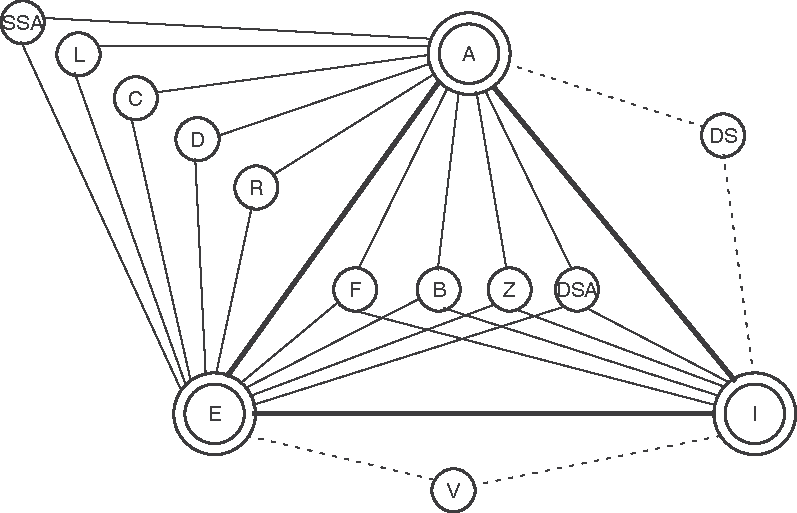
\includegraphics{Figure_12-1.pdf}
}{\caption{The aeroelastic triangle of forces.\label{fig12.1}}}}
\vspace*{-2\baselineskip}

It would be convenient to state concise definitions of each aeroelastic phenomenon which appears on the diagram in Fig. 1-1.

\textit{Flutter, F}. A dynamic instability occurring in an aircraft in flight at a speed called the flutter speed, where the elasticity of the structure plays an essential part in the instability.

\textit{Buffeting, B. }Transient vibrations of aircraft structural components due to aerodynamic impulses produced by the wake behind wings, nacelles, fuselage pods, or other components of the airplane.

\textit{Dynamic response, Z}. Transient response of aircraft structural components produced by rapidly applied loads due to gusts, landing, gun reactions, abrupt control motions, moving shock waves, or other dynamic loads.

\textit{Aeroelastic effects on stability, DSA \& SSA}. Influence of elastic deformations of the structure on dynamic and static airplane stability.

\textit{Load distribution, L}. Influence of elastic deformations of the structure on the distribution of aerodynamic pressures over the structure.

\textit{Divergence, D.} A static instability of a lifting surface of an aircraft in flight, at a speed called the divergence speed, where the elasticity of lifting surface plays an essential role in the instability.

\textit{Control effectiveness, C}. Influence of elastic deformations of the structure on the controllability of an airplane.

\textit{Control system reversal, R.} A condition occurring in flight, at a speed called the control reversal speed, at which the intended effects of displacing a given component of the control system are completely nullified by elastic deformations of the structure.

\textit{Mechanical vibrations, V.} A related field.

\textit{Dynamic stability, DS}. A related field.
\end{quote}
\vspace*{10pt}
\pagebreak

\section{Divergence analysis of a rigid wing segment}\label{sec12.2}
A model to illustrate the phenomenon of wing divergence consists of a uniform, rigid wing segment hinged to a fixed support in a wind tunnel as is shown in figure~\ref{fig12.2}. The hinge line is located at the \textbf{elastic axis} (E.A.) of the wing. The elastic axis coincides with the locus of shear centers of the wing sections.

Recall that the \textbf{shear center} of the cross section of a bar (wing) is a reference point in the cross section where the lateral deflections due to bending are de-coupled from the twist due to torsion (i.e., a shear force acting at the elastic axis results in bending deflections and no twist, and a torque acting at the elastic axis causes twist but no lateral deflection of the elastic axis due to bending).

The rigid wing segment is restrained against rotation, or twist, about the E.A. by a linear elastic rotational spring of stiffness $K$. This rotational spring is analogous the torsional stiffness per unit span, or $(G J)/L$, of a wing.

{\def\thefigure{12.2}
\processfigure{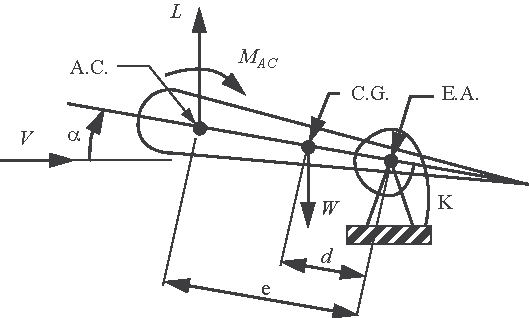
\includegraphics{Figure_12-2.pdf}
}{\caption{Rigid wing segment
model for divergence analysis\label{fig12.2}}}}


We assume two-dimensional, incompressible aerodynamics is applicable. Let $V$ denote the airspeed, $\alpha$ the angle of attack relative to the zero lift angle, $L$ the lift, $M_{A C}$ the pitching moment, and let $W$ denote the weight of the wing segment acting at the center of gravity (C.G.). The lift and pitching moment act at the aerodynamic center (A.C.), which is the point about which the pitching moment is independent of the angle of attack. Usually the A.C. is close to the quarter chord. We neglect the drag force $D$ relative to the lift since $D \ll L$.

The angle of attack is written\vspace*{-4pt} as
\begin{align}\label{eq12.1}
\alpha=\alpha_{0}+\theta,
\end{align}
where $\alpha_{0}$ is the initial wing incidence, or the angle of attack if there are no aerodynamic and gravity loads, and $\theta$ is the rotation angle due to elastic deformations of the spring. Assume small angles such that $\sin \alpha \approx \alpha$, $\cos \alpha \approx 1$, and $\tan \alpha \approx \alpha$. The lift is given\vspace*{-4pt} by
\begin{align}\label{eq12.2}
L=q S C_{L},
\end{align}
where $q$ is the dynamic pressure, $S$ is the wing planform area, and $C_{L}$ is the lift coefficient. Let $\rho$ denote the density of air, ${c}$ the chord length, and $s$ the wing span. The dynamic pressure, planform area, and lift coefficient are given~\vspace*{-4pt}by
\begin{align}\label{eq12.3}
q=\frac{1}{2} \rho V^{2} \quad S=c s \quad C_{L}=\left(\frac{\partial C_{L}}{\partial \alpha}\right) \alpha.
\end{align}
\vspace*{4pt}
\pagebreak

\noindent In the above equation $\left(\partial C_{L}\right) /(\partial \alpha)$ is the lift curve slope, which is assumed constant between stall points.

The pitching moment is given by
\begin{align}\label{eq12.4}
M_{A C}=q S c C_{\textit{MAC}},
\end{align}
where $C_{\textit{MAC}}$ is the pitching moment coefficient about the A.C., and is independent of $\alpha$.

Moment equilibrium about the E.A. gives
\begin{align}\label{eq12.5}
e L+M_{MAC}-W d-K \theta=0,
\end{align}
where $e$ is the distance from the E. A. to the A. C., assuming the E.A. is behind the A.C.

Substituting for the elastic twist, lift, and pitching moment from eqs. (\ref{eq12.1}) to (\ref{eq12.4}), the moment equation becomes
\begin{align}\label{eq12.6}
e q S\left(\frac{\partial C_{L}}{\partial \alpha}\right) \alpha+q S c C_{M A C}-W d-K\left(\alpha-\alpha_{0}\right)=0.
\end{align}
Rearrange eq.~(\ref{eq12.6}) to
\begin{align}\label{eq12.7}
\left[q S\left(\frac{\partial C_{L}}{\partial \alpha}\right) e-K\right] \alpha=W d-q S c C_{M A C}-K \alpha_{0}.
\end{align}
Now divide eq.~(\ref{eq12.7}) by $-K$ to get
\begin{align}\label{eq12.8}
\left[1-\frac{q S\left(\frac{\partial C_{L}}{\partial \alpha}\right) e}{K}\right] \alpha=\alpha_{0}-\frac{W d}{K}+\frac{q S c C_{M A C}}{K}.
\end{align}
Let
\begin{align}\label{eq12.9}
q_{D}=\frac{K}{S\left(\frac{\partial C_{L}}{\partial \alpha}\right) e}.
\end{align}
Hence, equation (\ref{eq12.8}) for the equilibrium value of the angle of attack reduces to
\begin{align}\label{eq12.10}
\alpha=\frac{\left[\alpha_{0}-(W d) / K+\Big(\frac{q}{q_{D}}\Big)\big(\frac{c}{e}\big) \frac{C_{M A C}}{\left(\frac{\partial C_{L}}{\partial \alpha}\right)}\right]}{1-q / q_{D}}.
\end{align}
A plot of $q / q_{D}$ versus the angle of attack obtained from eq.~(\ref{eq12.10}) is shown in figure~\ref{fig12.3}\vadjust{\vspace*{8pt}\pagebreak}.

{\def\thefigure{12.3}
\processfigure[H]{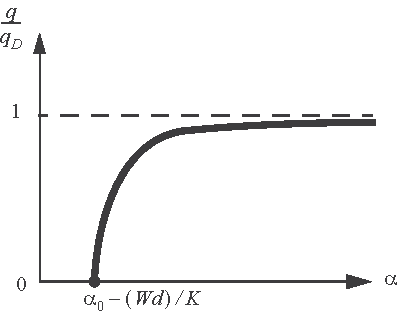
\includegraphics{Figure_12-3.pdf}
}{\caption{Response of the rigid wing segment model.\label{fig12.3}}}}


From eq.~(\ref{eq12.10}) we see that $\alpha \rightarrow \infty$ as $q \rightarrow q_{D}$ for $0 \leq q<q_{D}$. That is, the angle of attack grows without bound as $q \rightarrow q_{D}$. Of course, this excessive twist is a theoretical result. In reality the wing will stall or twist off due to a strength failure. Hence, the divergence dynamic pressure is defined as
\begin{align}\label{eq12.11}
q_{D}=\frac{K}{S\left(\frac{\partial C_{L}}{\partial \alpha}\right) e},
\end{align}
and the divergence speed is
\begin{align}\label{eq12.12}
V_{D}=\sqrt{\frac{2 q_{D}}{\rho}}.
\end{align}
Divergence corresponds to static instability. At $V=V_{D}$ we get excessive rotation in twist of the wing.


\subsection{Responses of the rigid wing segment and the imperfect column}\label{sec12.2.1}

The response plots of the rigid wing segment model of article \ref{sec12.2} and the geometrically imperfect column in article \ref{sec11.4} on page \pageref{sec11.4} are repeated in figure~\ref{fig12.4}. Comparing the two response plots reveals that these phenomena are the same. Both the column buckling and the wing divergence are static instabilities. The critical load $P_{\mathrm{cr}}$ for the column and the divergence dynamic pressure $q_{D}$ of the rigid wing segment model are determined from a static analysis of the slightly deflected structure.

{\def\thefigure{12.4}
\processfigure[H]{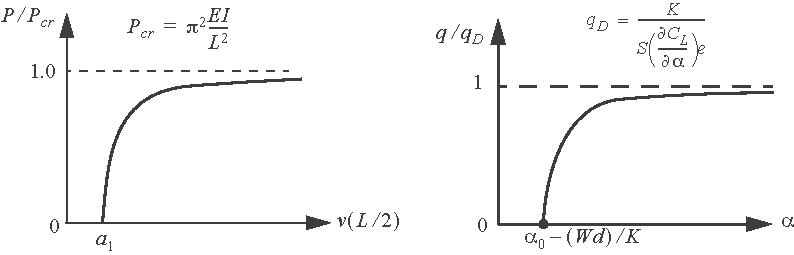
\includegraphics{Figure_12-4.pdf}
}{\caption{Response plots of the geometrically imperfect column and the rigid wing segment model.\label{fig12.4}}\vspace*{5pt}}}


\subsection{Divergence experiments}\label{sec12.2.2}


Experiments to measure the divergence dynamic pressure of an elastic wing confront the issue of damaging the wing and its supporting structure if the dynamic pressure is near or at its critical value. A nondestructive method to measure the critical dynamic pressure is accomplished by plotting the data on a Southwell plot, which was developed for elastic column buckling in article \ref{sec11.4.1} on page \pageref{sec11.4.1}. The Southwell plotting coordinates are determined from eq.~(\ref{eq12.10}) by formulating the change in the angle of attack $\Delta \alpha$, where $\Delta \alpha=\alpha-\left(\alpha_{0}-(W d) / K\right)$. After some algebraic manipulations, the change in the angle of attack is written as
\begin{align}\label{eq12.13}
\Delta \alpha=\frac{C_{0}\left(q / q_{D}\right)}{1-q / q_{D}},
\end{align}
where
\begin{align}\label{eq12.14}
C_{0}=\alpha_{0}-(W d) / K+\left(\frac{c}{e}\right) \frac{C_{M A C}}{\left(\frac{\partial C_{L}}{\partial \alpha}\right)}.
\end{align}
Equation (\ref{eq12.13}) is rearranged as follows: (1), Multiply each side by $1-q / q_{D}$, and write
\[
\Delta \alpha-\Delta \alpha\left(q / q_{D}\right)=C_{0}\left(q / q_{D}\right).
\]
(2) Divide by the dynamic pressure and write the final result as
\begin{align}\label{eq12.15}
\frac{\Delta \alpha}{q}=\frac{\left(\Delta \alpha+C_{0}\right)}{q_{D}}.
\end{align}

On the Southwell plot $(\Delta \alpha) / q$ is the ordinate and $\Delta \alpha$ is the abscissa. Thus, eq.~(\ref{eq12.15}) is a straight line on the plot as shown in figure~\ref{fig12.5}. The important aspect of the Southwell plot from the experimental viewpoint is that the slope of the graph is the reciprocal of the divergence dynamic pressure. As the dynamic pressure is increased from magnitudes less than the divergence dynamic pressure, the changes in angle of attack $\Delta \alpha$ become large, and the data of $(\Delta \alpha) / q$ versus $\Delta \alpha$ tends to plot as a straight line. The experimental divergence dynamic pressure is determined from the slope of this fitted straight line. The actual value of $C_{0}$ is not significant with respect to the determination of the experimental divergence dynamic pressure.

{\vspace*{-1\baselineskip}
\def\thefigure{12.5}
\processfigure[H]{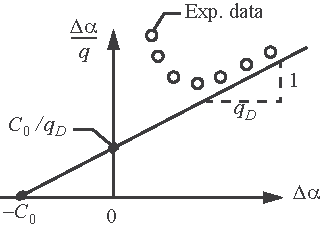
\includegraphics{Figure_12-5.pdf}
}{\caption{Southwell plot.\label{fig12.5}}\vspace*{-10pt}}
}

\vspace*{-15pt}
\section{Straight, uniform, unswept, high aspect ratio, cantilever wing in steady incompressible flow}\label{sec12.3}

Let $\alpha(z)$ denote the total wing incidence, and let $\alpha_{0}$ denote the fixed incidence at the wing root. The fixed incidence could be a function of $z$ for a variable in built-in twist, but we will consider it constant along the span. So
\begin{align}\label{eq12.16}
\alpha=\alpha_{0}+\phi_{z}(z),
\end{align}
\vspace*{2pt}\vspace*{-8pt}
\pagebreak

{\def\thefigure{12.6}
\processfigure[t]{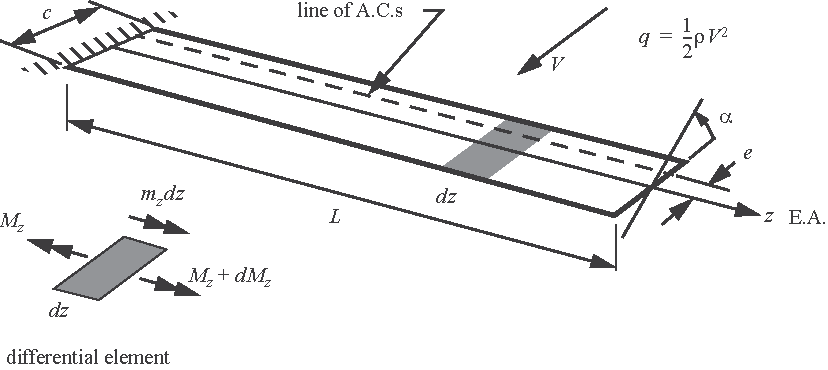
\includegraphics{Figure_12-6.pdf}
}{\caption{Wing model for torsional divergence analysis.\label{fig12.6}}}}

\noindent where $\phi_{z}(z)$ is the twist angle of the wing due to elastic deformation. Neglect airfoil weight, since we saw for the rigid wing segment that this factor played no role in the divergence dynamic pressure.

From eq.~(\ref{eq3.61}) on page \pageref{eq3.61} the differential equation in torsion is
\begin{align}\label{eq12.17}
\frac{d M_{z}}{d z}+m_{z}=0 \quad 0<z<L,
\end{align}
where $m_{z}$ denotes the external torque per unit span. In this case the external torque per unit span is due to the aerodynamic loads acting on the wing.

In reference to eq.~(\ref{eq3.121}) on page \pageref{eq3.121}, St. Venant's torsion theory relates the torque to the unit twist as
\begin{align}\label{eq12.18}
M_{z}=G J \frac{d \phi_{z}}{d z},
\end{align}
where $GJ$ is the torsional stiffness of the wing box. From eq.~(\ref{eq3.161}) page \pageref{eq3.161}, the torsion constant for a single-cell cross section is given by
\begin{align}\label{eq12.19}
J=\big(4 A_{c}^{2}\big) /\left(\oint \frac{d s}{t}\right),
\end{align}
where $A_{c}$ is the area enclosed by the cross-sectional contour, $s$ is the arc-length along the contour, and $t$ is the thickness of the contour. Substitute eq.~(\ref{eq12.18}) into (\ref{eq12.17}) and use the fact that the wing is uniform along the span to get
\begin{align}\label{eq12.20}
G J \frac{d^{2} \phi_{z}}{d z^{2}}+m_{z}=0 \quad \phi_{z}=\phi_{z}(z) \quad 0<z<L.
\end{align}

\subsection{Aerodynamic strip theory}\label{sec12.3.1}

Strip theory assumes aerodynamic lift and moment at station $z$ depends only on the angle of attack, or incidence, at $z$, and is independent of the angle of attack at any other spanwise locations. Physically, this is reasonable for high aspect ratio wings\vadjust{\vspace*{8pt}\pagebreak}.

{\def\thefigure{12.7}
\begin{figure}
\centering{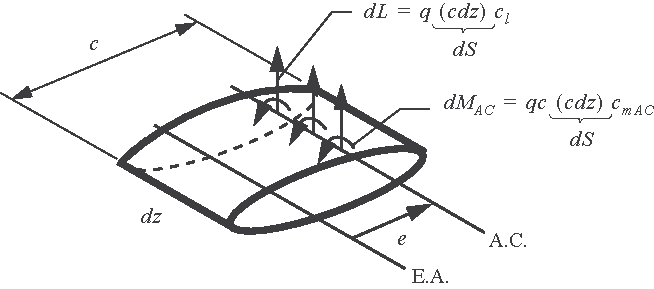
\includegraphics{Figure_12-7.pdf}}
\caption{Lift and pitching moment acting on the differential element of a wing.\label{fig12.7}}
\end{figure}
}


The differential lift and differential pitching moment acting at the A.C. on an typical element of the wing are shown in the figure~\ref{fig12.7}, where $c_{l}$ is the local lift coefficient and $C_{mAC}$ is the local moment coefficient about the A.C. Hence, the external torque acting on the differential element about the elastic axis is
\begin{align}\label{eq12.21}
m_{z} d z=e d L+d M_{A C}=\left[e q c c_{l}+q c^{2} c_{m A C}\right] d z,
\end{align}
or
\begin{align}\label{eq12.22}
m_{z}(z)=q c e c_{l}+q c^{2} c_{m A C}.
\end{align}
According to strip theory
\begin{align}\label{eq12.23}
c_{l}=\left(\frac{\partial c_{l}}{\partial \alpha}\right) \alpha=a_{0} \alpha,
\end{align}
where $a_{0}$ is the lift curve slope. Substituting eq.~(\ref{eq12.16}) into (\ref{eq12.23}), we get
\begin{align}\label{eq12.24}
c_{l}=a_{0}\left[\alpha_{0}+\phi_{z}(z)\right].
\end{align}
Hence,
\begin{align}\label{eq12.25}
m_{z}(z)=q c e a_{0}\left[\alpha_{0}+\phi_{z}(z)\right]+q c^{2} c_{m A C}.
\end{align}

\subsection{Differential equation of torsional divergence}\label{sec12.3.2}

Now substitute eq.~(\ref{eq12.25}) into (\ref{eq12.20}) and rearrange the terms to get
\begin{align}\label{eq12.26}
G J \frac{d^{2} \phi_{z}}{d z^{2}}+\left(q c e a_{0}\right) \phi_{z}=-q c e a_{0} \alpha_{0}-q c^{2} c_{m A C}.
\end{align}
Equation (\ref{eq12.26}) is the governing, second order, ordinary differential equation for $\phi_{z}(z)$ with $0<z<L$. The boundary conditions at $z=0$ and $z=L$ are to specify either $\phi_{z}$ or $M_{z}$, but not both. For a cantilever wing, which is clamped at the root and free at the tip, the boundary conditions are
\begin{align}\label{eq12.27}
\phi_{z}(0)=0 \quad M_{z}(L)=\left.G J \frac{d \phi_{z}}{d z}\right|_{z\,{=}\,L}=0.
\end{align}

The general solution of the ordinary differential eq.~(\ref{eq12.26}) is the sum of a particular solution and a homogenous solution.
\begin{align}\label{eq12.28}
\phi_{z}(z)=\phi_{p}(z)+\phi_{h}(z).
\end{align}
By the method of undetermined coefficients the particular solution is
\begin{align}\label{eq12.29}
\phi_{p}=-\alpha_{0}-\frac{c c_{m A C}}{e a_{0}}.
\end{align}

\vspace*{-1pc}

The homogenous equation is
\begin{align}\label{eq12.30}
G J \frac{d^{2} \phi_{h}}{d z^{2}}+\left(q c e a_{0}\right) \phi_{h}=0,
\end{align}
and its solution is given by
\begin{align}\label{eq12.31}
\phi_{h}=A_{1} \sin (\lambda z)+A_{2} \cos (\lambda z),
\end{align}
where
\begin{align}\label{eq12.32}
\lambda^{2}=\left(q c e a_{0}\right) /(G J).
\end{align}

Hence, the general solution for the wing twist is
\begin{align}\label{eq12.33}
\phi_{z}(z)=A_{1} \sin (\lambda z)+A_{2} \cos (\lambda z)-\alpha_{0}-\frac{c c_{m A C}}{e a_{0}}.
\end{align}
Substitute the general solution (\ref{eq12.33}) into the boundary conditions (\ref{eq12.27}) to determine constants $A_{1}$ and $A_{2}$:
\begin{align}\label{eq12.34}
A_{2}-\alpha_{0}-\frac{c c_{m A C}}{e a_{0}}=0 \quad A_{1} \lambda \cos (\lambda L)-A_{2} \lambda \sin (\lambda L)=0.
\end{align}
Solving eq.~(\ref{eq12.34}) for the constants, we get
\begin{align}\label{eq12.35}
A_{1}=\left(\alpha_{0}+\frac{c c_{m A C}}{e a_{0}}\right) \tan (\lambda L) \quad A_{2}=\alpha_{0}+\frac{c c_{m A C}}{e a_{0}}.
\end{align}
Substitute eq.~(\ref{eq12.35}) for ${A}_1$ and ${A}_2$ into eq.~(\ref{eq12.33}) to get the angle of twist for the cantilever wing as
\begin{align}\label{eq12.36}
\phi_{z}(z)=\left(\alpha_{0}+\frac{c c_{m A C}}{e a_{0}}\right)[\tan (\lambda L) \sin (\lambda z)+\cos (\lambda z)-1].
\end{align}

\vspace*{-1pc}

Hence from eqs. (\ref{eq12.16}) and (\ref{eq12.36}), the total wing incidence is
\begin{align}\label{eq12.37}
\alpha(z)=\alpha_{0}+\left(\alpha_{0}+\frac{c c_{m A C}}{e a_{0}}\right)\left[\frac{\sin (\lambda L) \sin (\lambda z)+\cos (\lambda L) \cos (\lambda z)}{\cos (\lambda L)}-1\right].
\end{align}
Using the trigonometric identity for the cosine of the sum of two angles, this last result can be written as
\begin{align}\label{eq12.38}
\alpha(z)=\alpha_{0}+\left(\alpha_{0}+\frac{c c_{m A C}}{e a_{0}}\right)\left[\frac{\cos [\lambda(L-z)]}{\cos (\lambda L)}-1\right].
\end{align}

From eq.~(\ref{eq12.38}) we see that $\alpha \rightarrow \infty$ if $\cos (\lambda L)=0$. Vanishing of the cosine function occurs when\break $\lambda L=\frac{\pi}{2}, 3 \frac{\pi}{2},\ldots.$ The lowest root gives the critical divergence dynamic pressure as
\begin{align}\label{eq12.39}
\left(\lambda_{D} L=\frac{\pi}{2}=\sqrt{\frac{q_{D} c e a_{0}}{G J} L}\right) \rightarrow q_{D}=\left(\frac{\pi}{2 L}\right)^{2} \frac{G J}{c e a_{0}}.
\end{align}
The value of $q_{D}$ in eq.~(\ref{eq12.39}) is the \textbf{wing's torsional divergence dynamic pressure}.

The analogy between the divergence dynamic pressure for the rigid wing model and the elastic wing model is summarized in table \ref{tab12.1}.

\begin{table}[H]
\processtable{Expressions for divergence dynamic
 pressure of the rigid wing and of the elastic wing\label{tab12.1}}{%
\tabcolsep=48pt\begin{tabular}{@{}ll@{}}
\toprule
\colhead{Rigid, eq.~(\ref{eq12.10})} & \colhead{Elastic, eq.~(\ref{eq12.39})}\\
\midrule
$K$ & $(G J) / L$\\
$S$ & $L c$\\
$e$ & $e$\\
$\left(\partial C_{L}\right) /(\partial \alpha)$ & $a_{0}$\\
\botrule
\end{tabular}}{}\vspace*{-10pt}
\end{table}

\vspace*{-16pt}
\section{Effect of wing sweep on divergence}\label{sec12.4}

Divergence of a slender straight wing that is approximately perpendicular to the airplane plane of symmetry is dependent on wing twist, referred to as torsional divergence, and bending is not a factor in the instability. For slender swept wings bending of the wing has an important and complicating affect on divergence and is referred to as bending-torsional divergence.


Let the angle $\Lambda$ denote the wing sweep measured relative to the unswept wing with $\Lambda>0$ for a swept-back wing, and $\Lambda<0$ for a swept-forward wing. See figure~\ref{fig12.8}. When a swept-back wing ($\Lambda>0$) bends, its angle of attack in the streamwise direction is reduced. Bending causes a nose-down twist in the streamwise direction. To understand this bending effect, consider an upward force applied to the reference axis. Points \textit{A} and \textit{B} deflect upward about the same amount. Point $A^{\prime}$ has less upward deflection since it is closer to the wing root.\begin{wrapfigure}[13]{l}{180pt}
\vspace{-6pt}
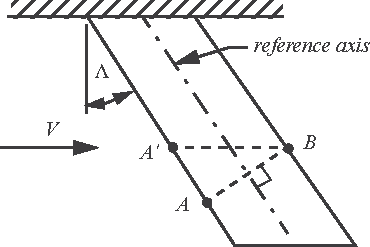
\includegraphics{Figure_12-8.pdf}
\caption{Streamwise and chordwise segments of a swept-back wing.\label{fig12.8}}
\end{wrapfigure} Hence, streamwise segment $A^{\prime} B$ will have a smaller angle of attack due to bending and a negative increment in lift results. This negative lift increment due to bending is a stabilizing influence, since it opposes the nose-up twist of segment $A^{\prime} B$.


Consider a swept-forward wing with $\Lambda<0$ as shown in figure~\ref{fig12.9}. Bending causes an increase in the angle of attack, or nose-up twist, for the streamwise segment $A^{\prime} B$. This increase in angle of attack due to bending is a destabilizing influence. Divergence essentially rules out swept-forward metallic wings. For wings made of composite materials, it is possible to materially couple bending and torsion in such a way to have an acceptable divergence speed for forward-swept wings (e.g., the X-29 demonstrator)\vadjust{\vspace*{8pt}\pagebreak}.

\begin{quote}
From NASA Armstrong Fact Sheet: X-29 Advanced Technology Demonstrator Aircraft (Gibbs, 2015): The X-29's thin supercritical wing was of composite construction. State-of-the-art composites permit aeroelastic tailoring, which allows the wing some bending but limits twisting and eliminates structural divergence within the flight envelope (deformation of the wing or breaking off in flight).
\end{quote}

{\def\thefigure{12.9}
\processfigure[H]{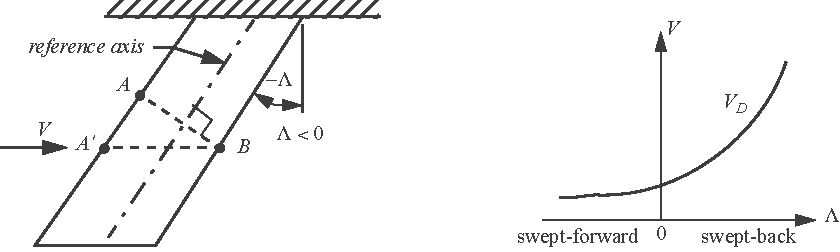
\includegraphics{Figure_12-9.pdf}
}{\caption{Streamwise and chordwise segments of a swept-forward wing.\label{fig12.9}}}}

\def\rightmark{Practice exercises}

\begin{thebibliography}{}\label{sec12.5}
\bibitem{}
Bisplinghoff, R.L., H. Ashley, and R.L. Halfman. \textit{\textbf{Aeroelasticity}}. Mineola, NY: Dover Publications, Inc., 1996. pp.~1--3, 421--432, 474 \& 475. (Originally published by Addison-Wesley, 1955.)

\bibitem{}
Gibbs, Y. ``NASA Armstrong Fact Sheet: X-29 Advanced Technology Demonstrator Aircraft.'' NASA.gov, November 5, 2015. \url{https://www.nasa.gov/centers/armstrong/news/FactSheets/FS-008-DFRC.html}.

\bibitem{}
Gordon, J. E. \textit{\textbf{Structures,} \textbf{or Why Things Don't Fall Down}}. Boston: Da Capo Press, 2003. (Originally published by Harmondsworth: Penguin Books. 1978.)
\end{thebibliography}

\section{Practice exercises}\label{sec12.6}

\begin{exercise}
\begin{enumerate}[\textbf{2.}]
\item[\textbf{1.}] An interesting historical account of wing torsional divergence is given by Gordon (2003); An excerpt follows.\vspace*{6pt}
\begin{splquote}
\hspace*{10pt}During World War I Antony Fokker developed an advanced monoplane fighter---the Fokker D8---with performance better than available or in immediate prospect on the Allied side. As soon as the D8 was flown in combat conditions it was found out that, when the aircraft was pulled out of a dive in a dog fight, the wings came off. Since many lives were lost---including those of some of the best and most experienced German fighter pilots---this was a matter of very grave concern to the Germans at the time, and is still instructive to study the cause of the trouble.\vspace*{1.6pt}
\end{splquote}

\bigskip

\hspace*{3pt}Read pages 260--271 in the book by Gordon and answer the following questions.
\begin{enumerate}[b)]
  \item[{\hskip13pt}a)] For a given engine power, why is a monoplane generally faster than a biplane?
  \item[{\hskip13pt}b)] What was the material of wing skin on the D8? Is it effective in resisting shear?
  \item[{\hskip13pt}c)] What was the method of loading in the structural test of the wings of the D8?
  \item[{\hskip13pt}d)] What was the ultimate load factor from the structural test?
  \item[{\hskip13pt}e)] What was the first attempt to strengthen the rear wing spar\vadjust{\vspace*{8pt}\pagebreak}?
  \item[{\hskip13pt}f)] What was the best method to strengthen the rear wing spar? and why did it work?
  \item[{\hskip13pt}g)] What is aileron reversal?
  \item[{\hskip13pt}h)] What common geometric feature do a tube and the torsion box of the old-fashioned biplane have that makes them so effective in resisting torsion?
\end{enumerate}



\item[\textbf{2.}] The uniform wing sketched in figure~\ref{fig12.10} is fixed at both ends. Starting with the general solution eq.~(\ref{eq12.33}), derive the algebraic expression for
\begin{enumerate}[b.]
  \item[{\hskip13pt}a.] total incidence $\alpha(z)=\alpha_{0}+\phi_{z}(z)$, and
  \item[{\hskip13pt}b.] divergence dynamic pressure $q_{D}$\vspace*{-10pt}.
  {\def\thefigure{12.10}

\processfigure[H]{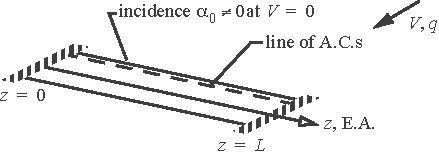
\includegraphics{Figure_12-10.pdf}
}{\caption{Wing with fixed ends.\label{fig12.10}}}}
\end{enumerate}



\item[\textbf{3.}] Consider a rigid wing segment of weight \textit{W} mounted on an elastic sting in a wind tunnel. The sting is modeled as a uniform, elastic, cantilever beam with bending stiffness $E I_{x x}=E I$ and length $2c$. Neglect the weight of the sting. The model is mounted in such a way to have the angle of attack $\alpha_{0}$ when the beam is undeformed. Thus, the angle of attack $\alpha=\alpha_{0}+\theta$, where $\theta$ is the nose-up rotation of the wing resulting from the bending of the sting. Denote the lift and the pitching moment acting at the aerodynamic center (A.C.) as \textit{L} and $M_{A C}$, respectively.

    {\def\thefigure{12.11}
\processfigure[H]{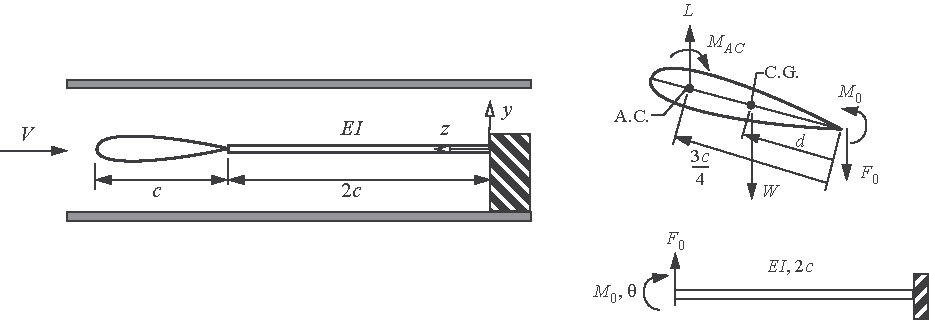
\includegraphics{Figure_12-11.pdf}
}{\caption{Rigid wing mounted on an elastic sting in a wind tunnel.\label{fig12.11}}}}


Assume
\begin{itemize}
  \item steady, two-dimensional incompressible flow at airspeed $V$ and density $\rho$,
  \item the lift curve slope $\frac{\partial C_{L}}{\partial \alpha}=a_{0}$ is constant between stall points,
  \item and that the angle of attack is small.
\begin{enumerate}[b.]
\item[\hspace*{-5.3pt}a.] Use the second theorem of Castigliano to determine the rotation $\theta$ of the cantilever beam due to end force $F_{0}$ and moment $M_{0}$ as shown in the sketch above. Consider bending only\vadjust{\vspace*{8pt}\pagebreak}.
  \item[\hspace*{-5.3pt}b.] Determine the angle of attack $\alpha$ as a function of the dynamic pressure $q=\left(\rho V^{2}\right) / 2$, $\alpha_{0}$, wing reference area \textit{S}, flexural stiffness \textit{EI}, chord length $c$, $a_{0}$, pitching moment coefficient $C_{\textit{MAC}}$, distance $d$, and weight \textit{W}.
  \item[\hspace*{-5.3pt}c.] Determine the divergence dynamic pressure, $q_{\mathrm{D}}$.
\end{enumerate}
\end{itemize}



\item[\textbf{4.}] A uniform beam with a rectangular cross section rests on a knife edge at its left end, while the right end is clamped in rigid disk. This configuration is shown in figure~\ref{fig12.12}. The bending stiffness $E I_{x x}=E I$, the distance between the knife edge and the beam's connection to the disk is \textit{L,} and the radius of the disk is $R$. This disk rotates about a fixed smooth pin through its center under the action of applied moment $M_a$ as shown. Determine the relation between the applied moment ${M_a}$ and rotation angle $\theta$ of the disk under the assumption that the angle of rotation $\theta$ is small. In a wind tunnel test the disk is connected to a rigid airfoil, then this structural configuration is used to provide the rotational spring of stiffness $K$ depicted in figure~\ref{fig12.2}.

       {\def\thefigure{12.12}
\processfigure[H]{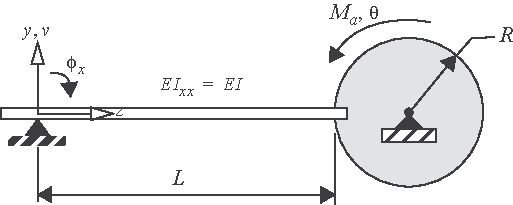
\includegraphics{Figure_12-12.pdf}
}{\caption{Apparatus to provide rota\-tional~stiffness in a wind tunnel test of an airfoil.\label{fig12.12}}}}


\end{enumerate}
\end{exercise}

\clearemptydoublepage

\end{document}